%
% einleitung.tex -- Beispiel-File für die Einleitung
%
% (c) 2020 Prof Dr Andreas Müller, Hochschule Rapperswil
%
\section{Modellierung von Populationen\label{logistic:section:einleitung}}
\rhead{Modellierung von Populationen}

Die logistische Gleichung ist ein beliebtes mathematisches Objekt,
das zeigt, wie aus einer scheinbar einfach Gleichung,
ein sehr komplexes und chaotisches Verhalten entstehen kann. 
Ihren Urpsrung hat die logistische Gleichung beim Modellieren
vom zeitlichen Verlauf von Populationen. 
Wie man dabei ganz organisch auf die logistische Gleichung 
kommt möchte ich hier kurz demonstrieren.

\medskip

Als erstens nehmen wir eine Population an, 
die ungehindert wachsen kann. 
Anfänglich hat diese die Tendenz, exponentiell zu wachsen. 
Ein einfaches mathematisches Modell für dieses Verhalten
könnte so aussehen:

\begin{equation}
    x_{n+1} = \lambda x_{n}
\end{equation}

\begin{figure}
    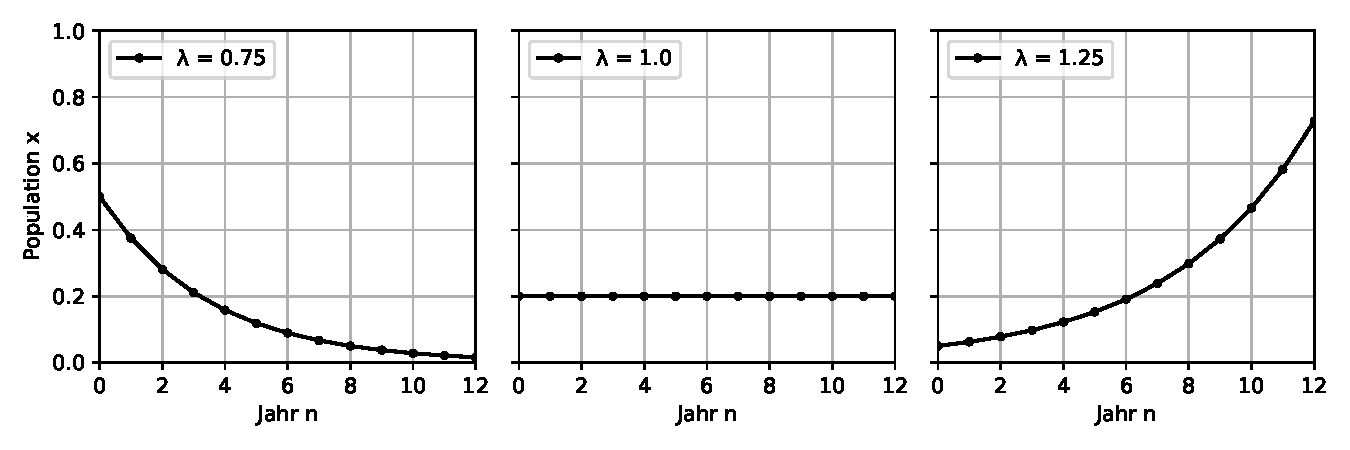
\includegraphics[width=\linewidth]{papers/logistic/figures/pop_exp.pdf}
    \caption{Exponentielle Populationsverläufe}
    \label{fig:pop_exp}
\end{figure}

Wobei $x_{n}$ die Population zu einem bestimmten Zeitpunkt ist, 
beispielsweise am Anfang vom Jahr $n$. 
Nun ist $x_{n+1}$ die Population im darauf folgenden Jahr. 
Der Faktor $\lambda$ gibt dabei an, wie schnell die Population
von Jahr zu Jahr ansteigt. 
Wenn $\lambda$ grösser als 1 ist,
wird die Population jedes Jahr grösser 
und wenn $\lambda$ kleiner als $1$ ist, 
wird die Population jedes Jahr kleiner.
Abbildung \ref{fig:pop_exp} zeigt das exponentielle 
Iterationsverhalten dieser Gleichung 
für einige Werte von $\lambda$. 


In der Realität können Populationen natürlich nicht endlos
exponentiell weiterwachsen, 
da früher oder später Platz, Nahrung, usw. ausgehen.
Um dieses Verhalten in das Modell zu implementieren,
fügen wir noch einen zusätzlichen Term hinzu, 
womit wir auch schon bei der logistischen Gleichung
angekommen sind:

\begin{equation}
    x_{n+1} = \lambda x_{n} (1 - x_{n})
\end{equation}

\begin{figure}
    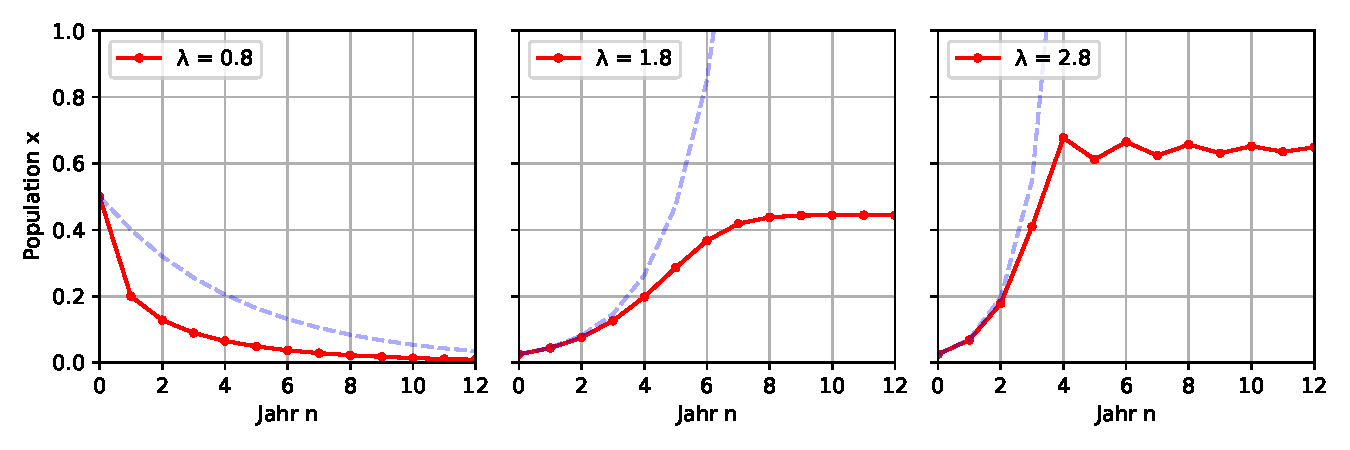
\includegraphics[width=\linewidth]{papers/logistic/figures/pop_logistic.pdf}
    \caption{Logistische Populationsverläufe}
    \label{fig:pop_logistic}
\end{figure}

Dieser Term sorgt dafür, 
dass das Wachstum der Population zurückgeht, 
wenn die sie grösser wird.
Der Wert von $x_n$ ist so limitiert auf 
$0 \le x_n \le 1$  
kann als die relative Population mit einem
theoretischen Maximum von 1 interpretiert werden. 
Abbildung \ref{fig:pop_logistic} zeigt das Iterationsverhalten 
der logistischen Gleichung für einige Werte von $\lambda$.




